
\documentclass{beamer}

\usepackage[utf8]{inputenc}
\usepackage[spanish]{babel}

\usepackage{beamerthemesplit}

\usetheme{Warsaw} 

\title{Redes neuronales multicapa}
\subtitle{Castiglione, Karpovsky, Sturla }
\author{Sistemas de Inteligencia Artificial}
\date{3 de Mayo de 2012}

\AtBeginSection[]
{
  \begin{frame}{Tabla de contenidos}
    \tableofcontents[currentsection]
  \end{frame}
}


\begin{document}

\frame{\titlepage}

\section[Outline]{}
\frame{\tableofcontents}

\section{Introducción}
\subsection{El problema}
\begin{frame}{El problema}

\par El problema planteado consiste en la estimación de funciones escalares a partir de un conjunto de puntos que las representan.
\vspace{10px}
\par En nuestor caso particular hemos trabajado con el archivo \textbf{samples7.txt}

\end{frame}

\begin{frame}{Gráfico de la función}

\begin{figure}[H]
\begin{center}
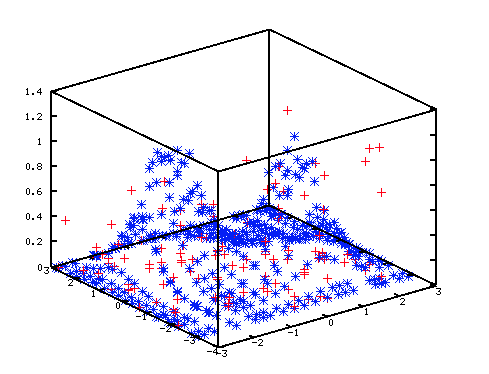
\includegraphics[scale=0.50]{./images/funcion.png}
\label{modelado}
\end{center}
\end{figure}

\end{frame}




\section{Modelado del problema}
\subsection{Representación de la red neuronal}

\begin{frame}{Representación de la red neuronal}
\par Se representó la red neuronal como una matriz de pesos. \\
\begin{itemize}
\item Cada neurona es una columna de pesos.
\item Cada capa de neuronas es una matriz de pesos.
\item La red neuronal, por consiguiente, es un vector de matrices.
\end{itemize}
\end{frame}

\subsection{Funciones de activación}
\begin{frame}
 Se utilizaron dos funciones de activación distintas:
\begin{block}{Sigmoidea exponencial}

\[
  g(h) = \frac{1}{1 + e^{-2 \beta h}} 
\]

Derivada:

\[
  2 \beta g(1-g) 
\]

\end{block}

\begin{block}{Tangente hiperbólica}

\[
  g(x) = tanh(x) 
\]

Derivada:

\[
  \beta g(1-g^2) 
\]

\end{block}

\end{frame}

\begin{frame}{Ruptura de la simetría}
\par asfas
\end{frame}


\subsection{Simetría}

\begin{frame}{Ruptura de la simetría}
\par asfsas
\end{frame}

\subsection{Cálculo del error}

\subsection{Conjuntos de entrenamiento y testeo}
\begin{frame}{Conjunto de entrenamiento y testeo}
\par Se decidió seguir el consejo de la cátedra y al realizar las pruebas se utilizó un subconjunto de los datos seleccionados al azar para la fase de aprendizaje y el subconjunto restante para testeo.

\begin{itemize}
\item Elección de puntos al azar? Puntos representativos?
\end{itemize}
\end{frame}

\section{Mejoras al algoritmo backpropagation}
\subsection{Eta dinámico}
\subsection{Ruido y momentum}

\section{Resultados}
\section{Conclusiones}
\begin{frame}{A sample slide}

\begin{theorem}[The Poincar\'e inequality]
Suppose $\Omega\in\mathbf{R}^n$ is a bounded domain with smooth
boundary.  Then there exists a $\lambda>0$, depending only on
$\Omega$, such that for any function $f$ in the Sobolev space
$H^1_0(\Omega)$ we have:

\[
  \int_\Omega |\nabla u|^2 \,dx \ge 
  \lambda \int_\Omega |u|^2 \,dx .
\]
\end{theorem}

Here is what \emph{itemized} and \emph{enumerated} lists look like:

\begin{columns}
  \begin{column}{0.45\textwidth}
  \begin{itemize}
    \item itemized item 1
    \item itemized item 2
    \item itemized item 3
  \end{itemize}
  \end{column}

  \begin{column}{0.45\textwidth}
  \begin{enumerate}
    \item enumerated item 1
    \item enumerated item 2
    \item enumerated item 3
  \end{enumerate}
  \end{column}
\end{columns}

\end{frame}

\end{document}
